Nach erfolgreicher EDX-Analyse wurden die folgenden Daten erfasst:


\begin{table}[H]
  \centering

\adjustbox{max width=\textwidth}{

% Resize the table to fit within the page
%\resizebox{\textwidth}{!}{%


\renewcommand{\arraystretch}{1.7} % Increase row height (local)
\fontsize{18pt}{20pt}\selectfont
  \begin{tabular}{|l|l|c|c|}
  \hline
  \textbf{Bereich}          & \textbf{Element} & \multicolumn{1}{l|}{\textbf{Atomare Konz. {[}\%{]}}} & \multicolumn{1}{l|}{\textbf{Gewichtskonz. {[}\%{]}}} \\ \hline
  \textbf{Gate Pad}         & Au               & 84,49                                                & 92,57                                                \\
  \textbf{}                 & Pd               & 10,05                                                & 5,95                                                 \\
  \textbf{}                 & Ni               & 3,49                                                 & 1,14                                                 \\ \hline
  \textbf{Sinterpad rechts} & C                & 83,77                                                & 69,68                                                \\
  \textbf{}                 & Al               & 16,23                                                & 30,32                                                \\ \hline
  \textbf{Sinterpad rechts} & Al               & 97,92                                                & 92,19                                                \\
  \textbf{}                 & Ag               & 2,08                                                 & 7,81                                                 \\ \hline
  \textbf{Sinterpad links}  & Ag               & 69,80                                                & 95,40                                                \\
  \textbf{}                 & C                & 30,20                                                & 4,60                                                 \\ \hline
  \textbf{Source Pad}       & Au               & 81,91                                                & 91,26                                                \\
  \textbf{}                 & Pd               & 11,41                                                & 6,87                                                 \\
                            & Ni               & 4,50                                                 & 1,50                                                 \\ \hline
  \textbf{Source Pad}       & Au               & 80,60                                                & 90,70                                                \\
                            & Pd               & 11,46                                                & 6,97                                                 \\
                            & Ni               & 5,87                                                 & 1,97                                                 \\ \hline
  \textbf{Tiegel}           & Al               & 100,00                                               & 100,00                                               \\ \hline
  \end{tabular}}
  \caption{EDX-Analyse der untersuchten Bereiche}
  \label{Tab. 1}
  \end{table}
    

  \subsection{GatePad}
    \begin{figure}[H]
        \centering
        \begin{minipage}{.5\textwidth}
          \centering
          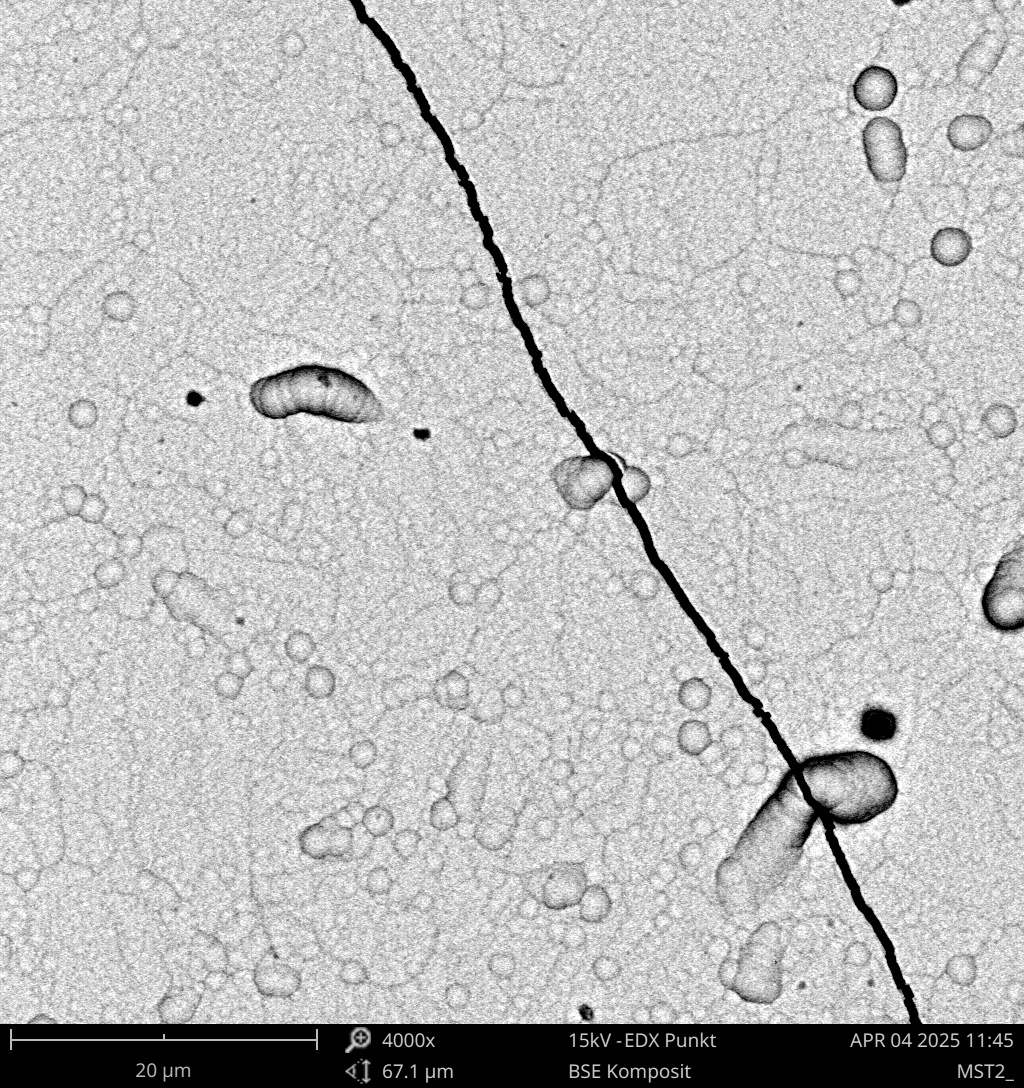
\includegraphics[width=.9\linewidth]{Bilder/MST2_0002}
          \captionof{figure}{REM-Aufnahme(BSE Komposit, 4000x, 67,5 \si{\micro\meter}) des GatePads mit Punktanalyse, (Selbsterstellte Abbildungen)}
          \label{Abb.2: REM-Aufnahme(BSE Komposit, 4000x) des GatePads mit Punktanalyse}
        \end{minipage}%
        \begin{minipage}{.5\textwidth}
          \centering
          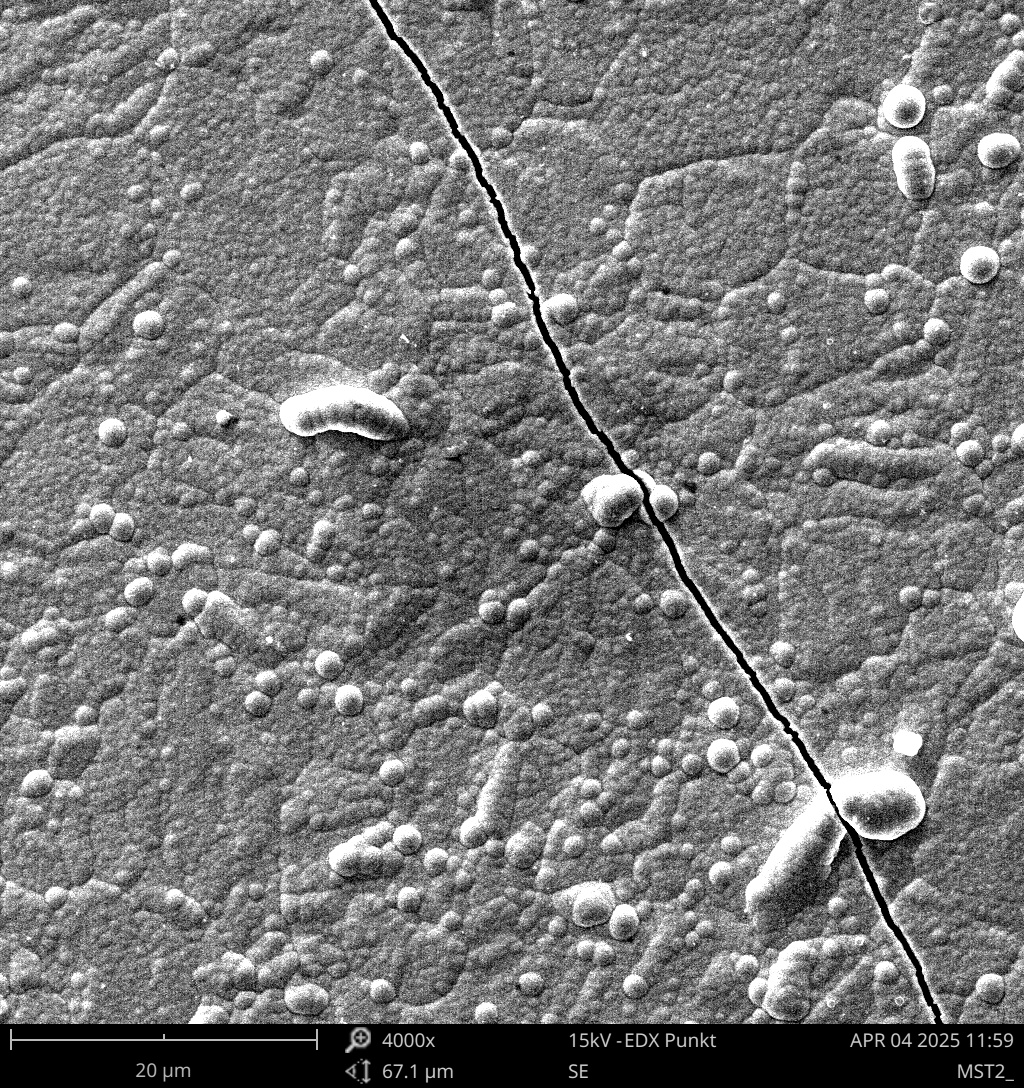
\includegraphics[width=.9\linewidth]{Bilder/MST2_0005}
          \captionof{figure}{REM-Aufnahme(SE Komposit, 4000x, 67,5 \si{\micro\meter}) des GatePads mit Punktanalyse, (Selbsterstellte Abbildungen)}
          \label{REM-Aufnahme(SE Komposit) des GatePads mit Punktanalyse}
        \end{minipage}
        
        \end{figure}
        \begin{figure}[H]
            \centering
            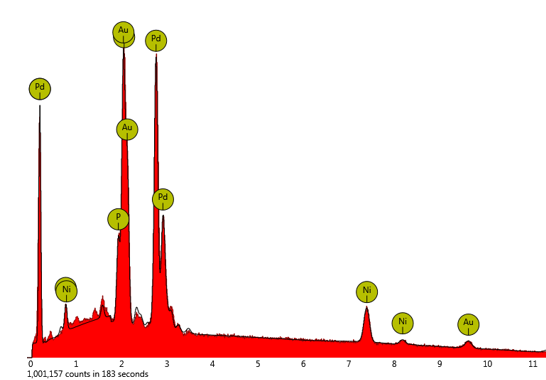
\includegraphics[scale=0.95]{Bilder/gatepad}
            \caption{EDX Analyse des GatePads mit Darstellung der chemischen Zusammensetzung der Elemente, (Phenom erstellte Bericht)}
            
            \vspace{0.2cm}
            \label{Abb.2: EDX Analyse des GatePads}
        \end{figure} 
        Im BSE-Bild des GatePads lassen sich deutlich helle Flächen erkennen, die auf einen hohen Anteil von Gold hinweisen. Laut EDX-Analyse besteht die Oberfläche zu etwa 92,57 \% aus Gold, ergänzt durch rund 5,95 \% Palladium und 1,14 \% Nickel. Die Fläche erscheint insgesamt glatt und homogen, mit nur wenigen sichtbaren Einschlüssen und feinen Rissen.

        Das SE-Bild gibt dagegen detaillierte Einblicke in die Topografie. Hier zeigen sich partikuläre Strukturen und kleine Oberflächendefekte. Zudem sind leichte Kantenkontraste sowie kugelartige Erhebungen erkennbar, die auf eine unregelmäßige Oberflächenstruktur hindeuten.

\subsection{Sinterpad rechts}
    \begin{figure}[H]
        \centering
        \begin{minipage}{.5\textwidth}
          \centering
          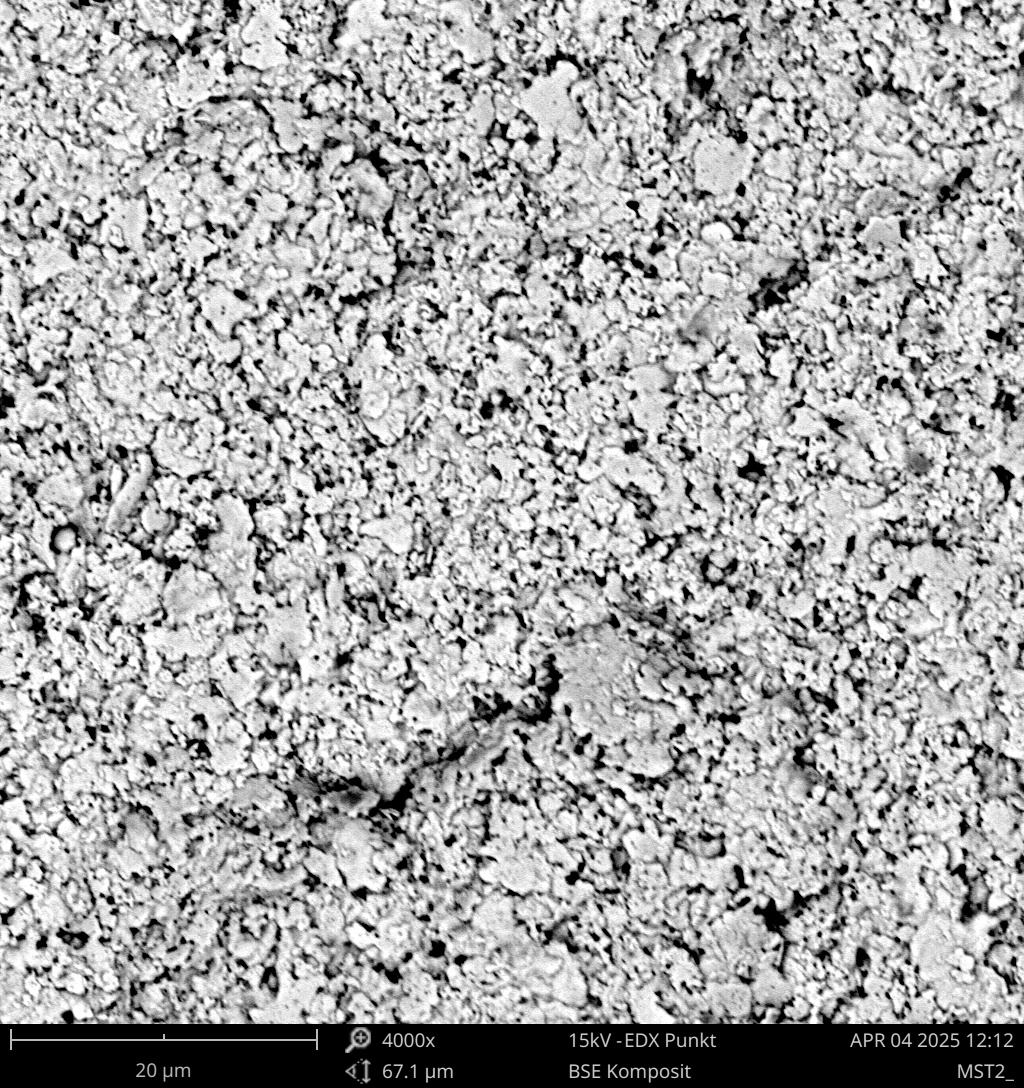
\includegraphics[width=.9\linewidth]{Bilder/MST2_0013}
          \captionof{figure}{REM-Aufnahme(BSE Komposit, 4000x, 67,5 \si{\micro\meter}) des SinterPads rechts mit Punktanalyse, (Selbsterstellte Abbildungen)}
          \label{Abb.2: REM-Aufnahme(BSE Komposit, 4000x) des SinterPads rechts mit Punktanalyse}
        \end{minipage}%
        \begin{minipage}{.5\textwidth}
          \centering
          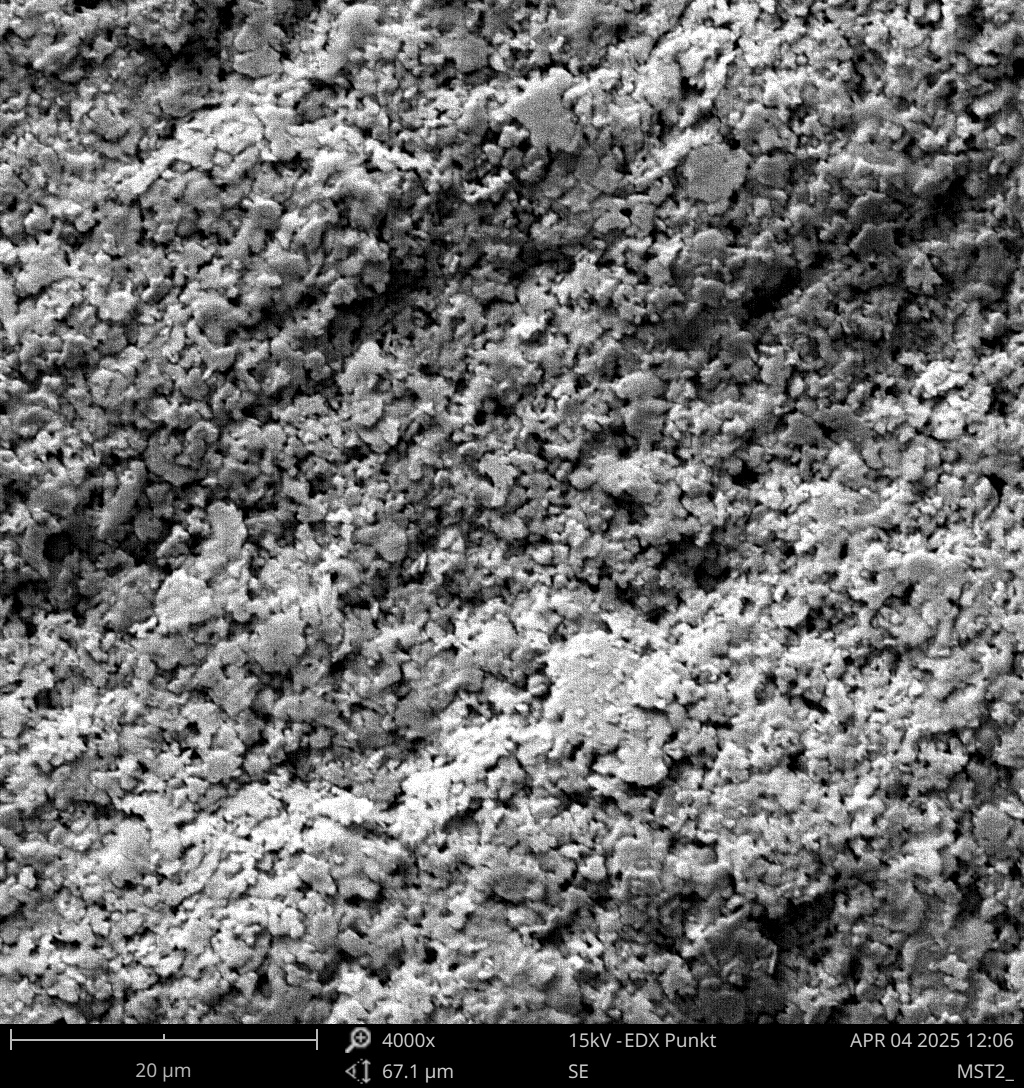
\includegraphics[width=.9\linewidth]{Bilder/MST2_0010}
          \captionof{figure}{REM-Aufnahme(SE Komposit, 4000x, 67,5 \si{\micro\meter}) des SinterPads rechts mit Punktanalyse, (Selbsterstellte Abbildungen)}
          \label{REM-Aufnahme(SE Komposit, 4000x) des SinterPads rechts mit Punktanalyse}
        \end{minipage}
        
        \end{figure}
        \begin{figure}[H]
            \centering
            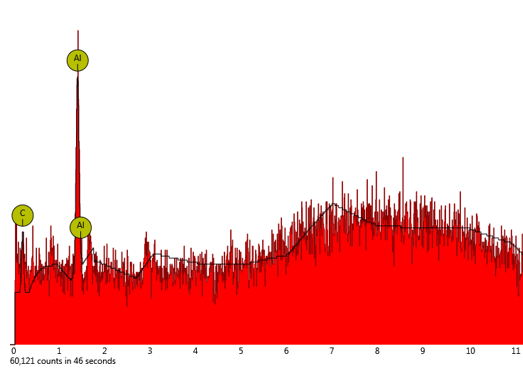
\includegraphics[scale=0.95]{Bilder/sinterpadrechts}
            \caption{EDX Analyse des SinterPads rechts mit Darstellung der chemischen Zusammensetzung der Elemente, (Phenom erstellte Bericht)}
            
            \vspace{0.2cm}
            \label{Abb.2: EDX Analyse des SinterPads rechts}
        \end{figure} 
        Die SE-Aufnahme des rechten Sinterpads zeigt eine stark poröse und grobkörnige Oberfläche. Die Partikel sind ungleichmäßig verteilt und variieren deutlich in ihrer Größe. Das lässt darauf schließen, dass der Bereich nur teilweise gesintert wurde. Die EDX-Analyse unterstützt diese Beobachtung mit einem hohen Kohlenstoffanteil (83,77 \%) und etwa 16,23 \% Aluminium.

        Im BSE-Bild erscheint die Fläche weitgehend gleichmäßig hell. Dies deutet darauf hin, dass keine deutlichen Cluster von Elementen mit hoher Ordnungszahl vorhanden sind. Die gleichmäßige Helligkeit lässt sich mit der homogenen Verteilung von Aluminium und Kohlenstoff erklären, wobei Silber in diesem Bereich nicht nachgewiesen wurde.

\subsection{SourcePad}
    \begin{figure}[H]
        \centering
        \begin{minipage}{.5\textwidth}
          \centering
          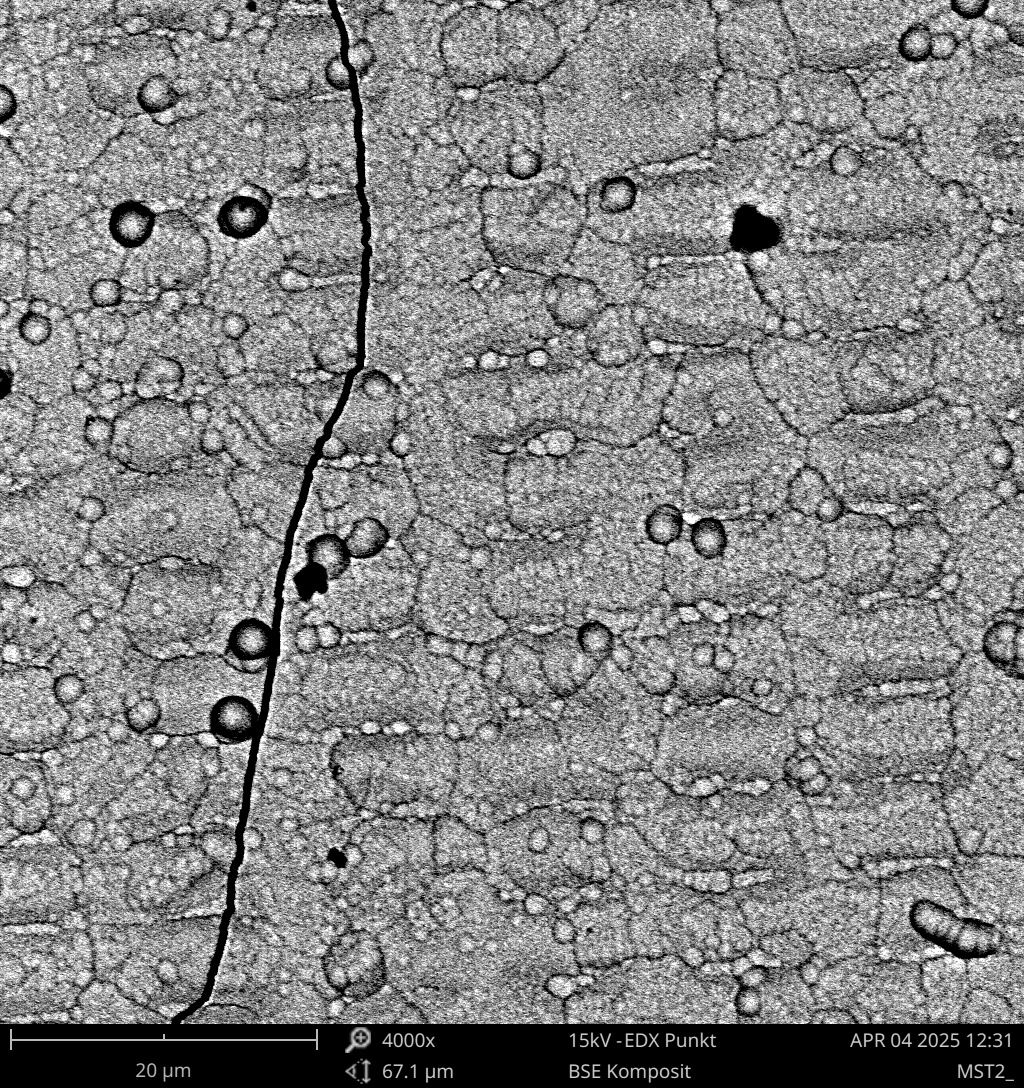
\includegraphics[width=.9\linewidth]{Bilder/MST2_0019}
          \captionof{figure}{REM-Aufnahme(BSE Komposit, 4000x, 67,5 \si{\micro\meter}) des SourcePads mit Punktanalyse, (Selbsterstellte Abbildungen)}
          \label{Abb.2: REM-Aufnahme(BSE Komposit, 4000x) des SourcePads mit Punktanalyse}
        \end{minipage}%
        \begin{minipage}{.5\textwidth}
          \centering
          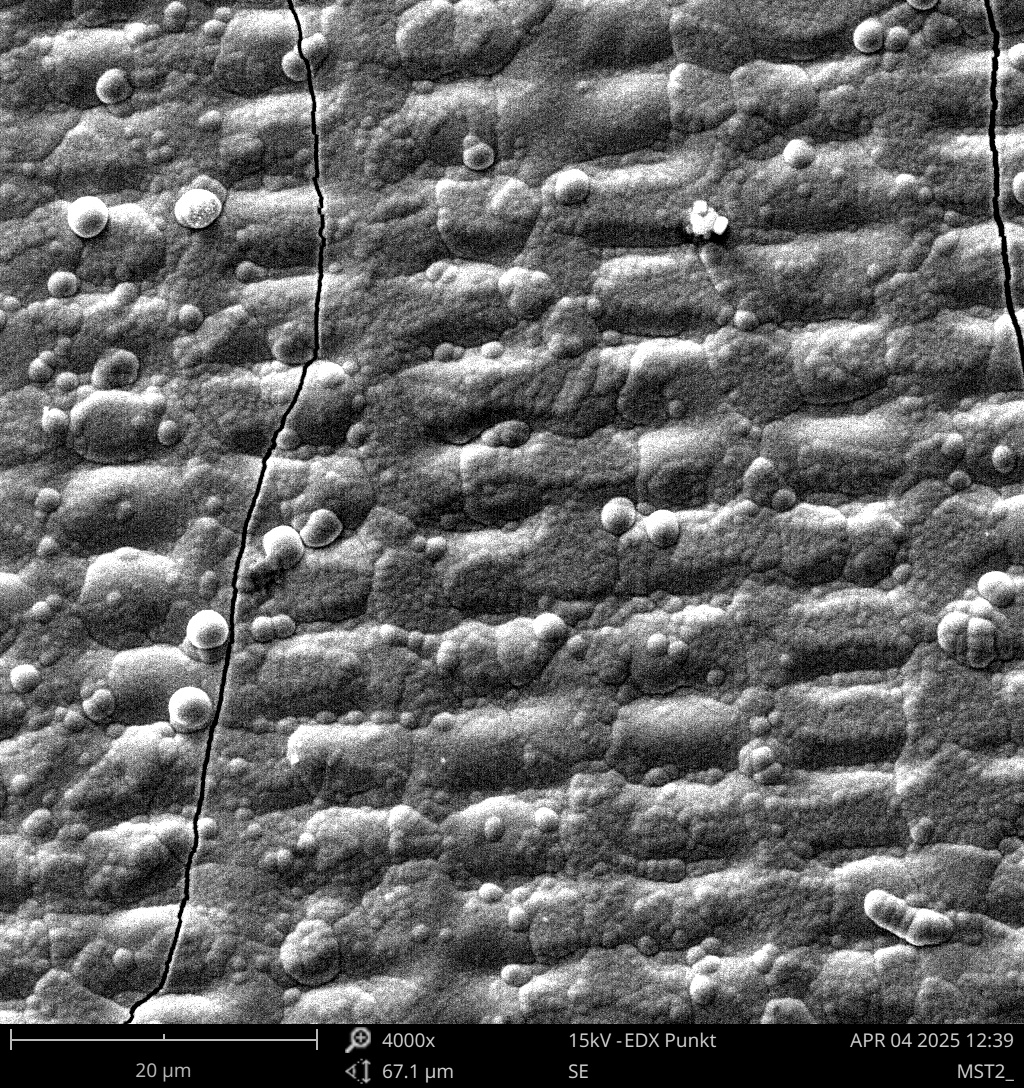
\includegraphics[width=.9\linewidth]{Bilder/MST2_0022}
          \captionof{figure}{REM-Aufnahme(SE Komposit, 4000x, 67,5 \si{\micro\meter}) des SourcePads mit Punktanalyse, (Selbsterstellte Abbildungen)}
          \label{REM-Aufnahme(SE Komposit, 4000x) des SourcePads mit Punktanalyse}
        \end{minipage}
        
        \end{figure}
        \begin{figure}[H]
            \centering
            \includegraphics[scale=0.95]{Bilder/SourcePad}
            \caption{EDX Analyse des SourcePads mit Darstellung der chemischen Zusammensetzung der Elemente, (Phenom erstellte Bericht)}
            
            \vspace{0.2cm}
            \label{Abb.2: EDX Analyse des SourcePads}
        \end{figure}
        Im BSE-Modus zeigt das SourcePad einen starken Kontrast, der auf die Anteile von Gold und Palladium zurückzuführen ist. Die Analyse belegt eine sehr homogene Verteilung dieser Elemente, ergänzt durch feine Risse und punktuelle Einschlüsse in der Struktur.

        Die SE-Aufnahme offenbart eine deutlich strukturierte Oberfläche mit einer streifenförmigen Textur. Die zahlreichen kleinen Partikel auf der Oberfläche könnten durch Diffusions- oder Herstellungsprozesse entstanden sein. Diese feinen topografischen Merkmale lassen Rückschlüsse auf die Qualität der Metallisierung zu.

\subsection{Tiegel}
    \begin{figure}[H]
        \centering
        \begin{minipage}{.5\textwidth}
          \centering
          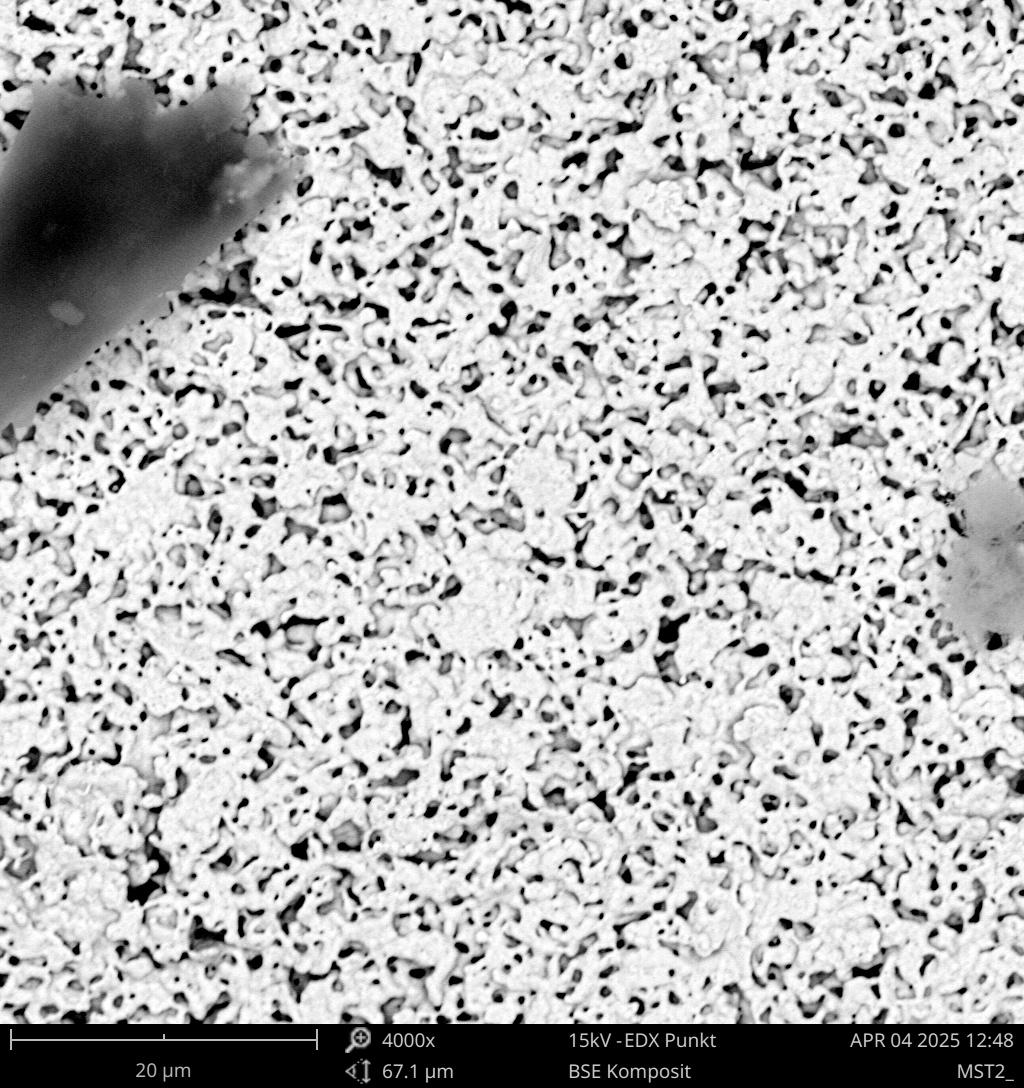
\includegraphics[width=.9\linewidth]{Bilder/MST2_0029}
          \captionof{figure}{REM-Aufnahme(BSE Komposit, 4000x, 67,5 \si{\micro\meter}) des Tiegels mit Punktanalyse, (Selbsterstellte Abbildungen)}
          \label{Abb.2: REM-Aufnahme(BSE Komposit, 4000x) des Tiegels mit Punktanalyse}
        \end{minipage}%
        \begin{minipage}{.5\textwidth}
          \centering
          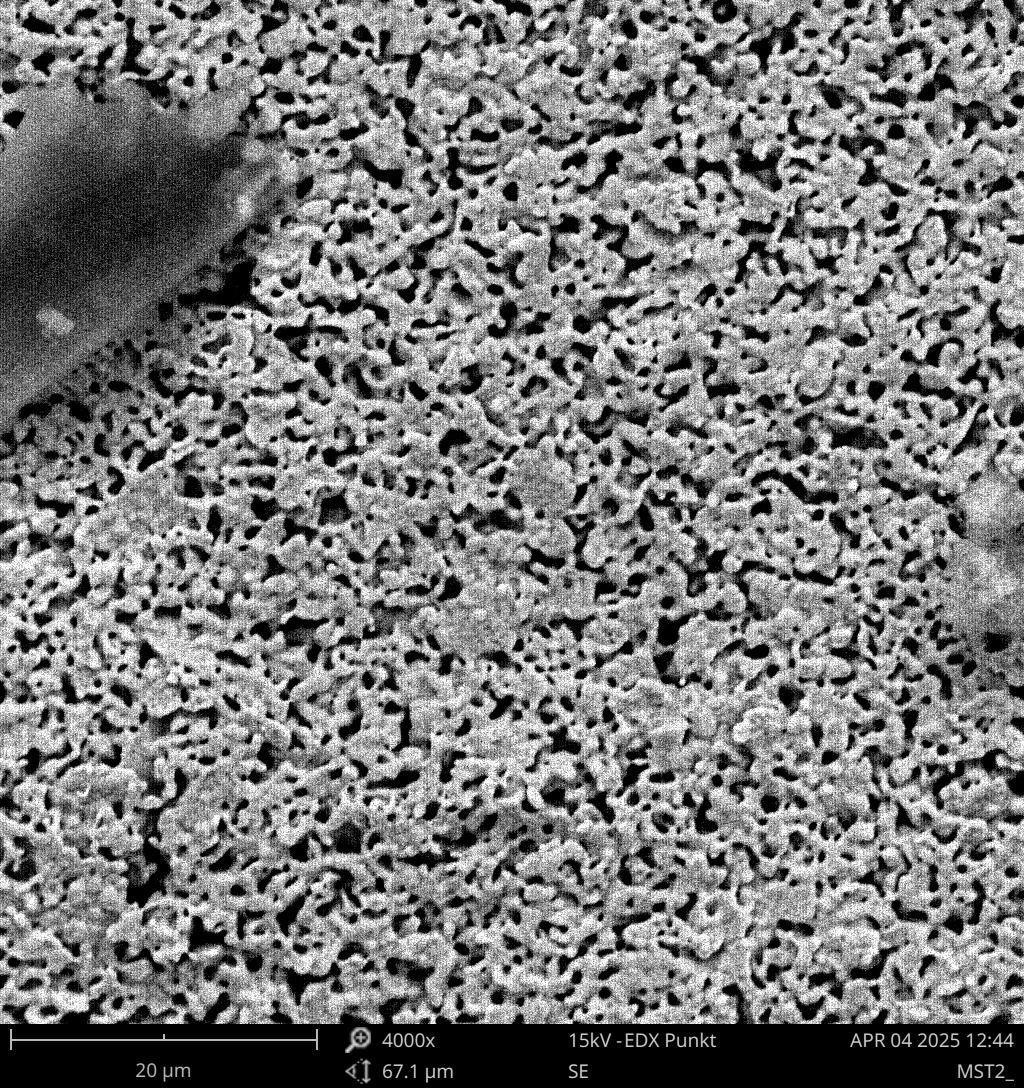
\includegraphics[width=.9\linewidth]{Bilder/MST2_0026}
          \captionof{figure}{REM-Aufnahme(SE Komposit, 4000x, 67,5 \si{\micro\meter}) des Tiegels mit Punktanalyse, (Selbsterstellte Abbildungen)}
          \label{REM-Aufnahme(SE Komposit, 4000x) des Tiegels mit Punktanalyse}
        \end{minipage}
        
        \end{figure}
        \begin{figure}[H]
            \centering
            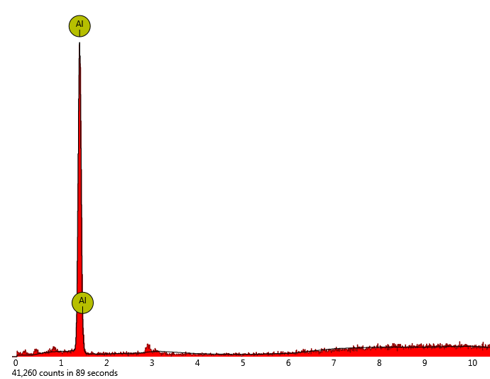
\includegraphics[scale=0.95]{Bilder/tiegel}
            \caption{EDX Analyse des Tiegels mit Darstellung der chemischen Zusammensetzung der Elemente, (Phenom erstellte Bericht)}
            
            \vspace{0.2cm}
            \label{Abb.2: EDX Analyse des Tiegels}
        \end{figure}
        Im SE-Bild vom Tiegel ist eine schwammartige, poröse Struktur zu erkennen. Die Poren sind recht gleichmäßig verteilt, was auf ein gesintertes Aluminium-Material hindeutet. Auf der linken Seite des Bildes sieht man außerdem einen größeren Fremdkörper, der sich vom Rest deutlich abhebt.

Das BSE-Bild zeigt eine gleichmäßig helle Fläche, was gut zu den EDX-Ergebnissen passt: 100 \% Aluminium, keine anderen Elemente nachweisbar. Das spricht für eine sehr homogene Zusammensetzung.